
\documentclass[12pt,a4paper,titlepage,oneside]{article}
\usepackage[top=2.5cm, bottom=2cm, left=2.5cm, right=1cm]{geometry} 
% Font, accents
\usepackage[utf8]{inputenc}
\usepackage{fancyhdr}
\usepackage[T1]{fontenc}
\usepackage{times}     
% Interactive index
\usepackage{hyperref}
% Spanish titles
\usepackage[spanish]{babel}
% Attached files
\usepackage{attachfile}
\attachfilesetup{
  icon = Paperclip
}
% Fix curly verbatim apostrophes
\usepackage{upquote,textcomp}
% Make lists without bullets
\renewenvironment{itemize}{
 \begin{list}{}{
  \setlength{\leftmargin}{1.5em}
 }
}{
 \end{list}
}



%Customize things
\usepackage[margin=0pt,font=small,labelfont=bf]{caption}
\usepackage{graphicx}
\usepackage[usenames,dvipsnames]{xcolor}

% Sections and subsections colors
\usepackage{titlesec}
\titleformat{\section}
{\color{Blue}\normalfont\Large\bfseries}
{\color{Blue}\thesection}{1em}{}
\newcommand{\sectionbreak}{\clearpage}


% Document properties
\title{Facultad de Ingeniería\\Técnicas de Programación Concurrente I [75.59]}
\date{\today}
\hypersetup{
  colorlinks = true,
  urlcolor=blue,
  pdflang = es,
  pdfauthor = {Federico Farina},
  pdfproducer = {Federico Farina},
  pdfcreator = Texmaker,
  pdftitle = {TP1},
}

\begin{document}
   % code start
    \fancyhead[LE]{\leftmark} 
    \fancyhead[RO]{\rightmark} 
    \fancyhead[L]{Técnicas de Programación Concurrente I}
    \fancyhead[R]{TP1}    
    \renewcommand{\headrulewidth}{0.4pt} 
    \renewcommand{\footrulewidth}{0pt}
    % code end

    % set pagestyle to use fancy header and footer
    \pagestyle{fancy}


 \maketitle
  \setcounter{page}{1}
  \pagenumbering{roman}
  \tableofcontents

\newpage{}
\pagenumbering{arabic}
\setcounter{page}{1}

\section{Enunciado}

\subsection{Objetivo}

El objetivo de este proyecto consiste en implementar la simulación parcial del funcionamiento de una estación de servicio.

\subsection{Requerimientos Funcionales}

Esta simulacion abarcar a el funcionamiento de una estación de servicio. Los requerimientos funcionales son los siguientes:

\begin{enumerate}
\item 
La estacion de servicio cuenta con un número determinado de surtidores, un jefe de estación y un conjunto de empleados que atienden de a un auto por vez.
\item 
Tanto el número de surtidores disponibles como el número de empleados deben ser configurables y se establecen al inicio de la simulación.
\item
Cuando un auto llega a la estación de servicio es atendido en primer lugar por el jefe de estación quien asignará un empleado para atender al auto. Si no hay un empleado disponible, el auto se retira de la estación de servicio.
\item
El jefe de estación debe atender a los autos por orden de llegada de los mismos.
\item
Cuando el empleado recibe un auto de parte del jefe de estación, debe localizar un surtidor libre para atender al auto en cuestión. Si no encuentra ningú surtidor libre, deberá esperar hasta tanto se libere alguno.
\item
Una vez que el empleado obtiene un surtidor atiende al auto en cuestión. Mientras el empleado está atendiendo al auto no se puede utilizar el mismo surtidor para otro auto, ni el empleado es capaz de atender más de un auto a la vez.
\item
Finalmente, antes de que el auto se retire el empleado deberá cobrar el cargo correspondiente, el cual será almacenado en la caja de la estación de servicio.
\item
Todos los empleados guardan la recaudación en la misma caja y sólo un empleado puede utilizar la caja a la vez.
\item
Durante cualquier momento de la simulación, el administrador de la estación de servicio podrá consultar la recaudación guardada en la caja. Mientras lo hace, si algún empleado tiene recaudación para guardar, deberá esperar hasta que el administrador finalice su consulta.
\end{enumerate}

 
\subsection{Requerimientos no Funcionales}

Los siguientes son los requerimientos no funcionales de la aplicación:

\begin{enumerate}
 \item
  El proyecto deberá ser desarrollado en lenguaje C o C++, siendo este último el  lenguaje de preferencia.
  \item
  La simulación puede no tener interfaz gráfica y ejecutarse en una o varias consolas de línea decomandos.
  \item
  El proyecto deberá funcionar en ambiente Unix / Linux.
  \item
La aplicación deberá funcionar en una única computadora.  
\item
El programa deberá poder ejecutarse en "modo debug", lo cual dejará registro de la actividad que realiza en un único archivo de texto para su revisión posterior.
\end{enumerate} 


Las facilidades de IPC que se podrán utilizar para la realización de este proyecto son las que abarcan la primera parte de la materia, es decir, hasta el primer parcial. Dichas facilidades son: 
\begin{itemize}
\item[•] Memoria compartida
\item[•] Señales
\item[•] Pipes y fifos
\item[•] Locks
\item[•] Semaforos
\end{itemize}

Cualquier otra facilidad queda expresamente excluida para este proyecto.

\subsection{Tareas a Realizar}

A continuación se listan las tareas a realizar para completar el desarrollo del proyecto:

\begin{enumerate}
\item
 Dividir el proyecto en procesos. El objetivo es lograr que la simulación esté conformada por un conjunto de procesos que sean lo más sencillos posible.
\item
Una vez obtenida la división en procesos, establecer un esquema de comunicación entre ellos teniendo en cuenta los requerimientos de la aplicación. ¿Qué procesos se comunican entre sí?, ¿Qué datos necesitan compartir para poder trabajar?
\item
Tratar de mapear la comunicación entre los procesos a los problemas conocidos de concurrencia.
\item 
Determinar los mecanismos de concurrencia a utilizar para cada una de las comunicaciones entre procesos que fueron detectadas en el ítem 2. No se requiere la utilización de algún mecanismo específico, la elección en cada caso queda a cargo del grupo y debe estar debidamente justificada.
\item
 Realizar la codificación de la aplicación. El código fuente debe estar documentado.
\end{enumerate}
 
\subsection{Entrega} 

La entrega del proyecto comprende lo siguiente:

\begin{enumerate}
\item
Informe, se deberá presentar impreso en una carpeta o folio y en forma digital (PDF) a través del campus
\item
El código fuente de la aplicación, que se entregará únicamente mediante el campus
\end{enumerate}

La entrega en el campus estará habilitada hasta las 19 hs de la fecha indicada oportunamente.

El informe a entregar debe contener los siguientes ítems:

\begin{enumerate}
\item
Breve análisis del problema, incluyendo una especificación de los casos de uso de la aplicación.
\item
Detalle de resolución de la lista de tareas anterior.
\item
Diagrama que refleje los procesos, el flujo de comunicación entre ellos y los datos que intercambian.
\item
Diagramas de clases realizados.
\item
Diagrama de transición de estados del jefe de estación.
\end{enumerate}

\section{Diagrama de Clases}
\begin{figure}[hbtp]
\centering
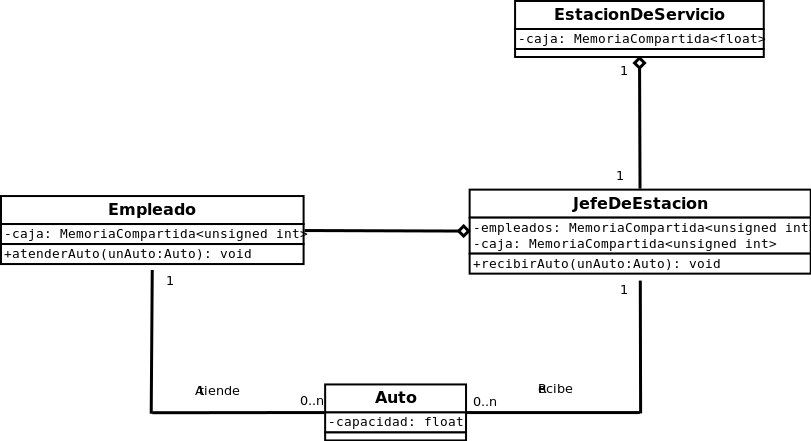
\includegraphics[scale=0.5]{diagramaDeClases.png}
\caption{Diagrama de Clases}
\end{figure}

\section{Casos de Uso}


\end{document}